\section{Eigenvalues and Eigenvectors} \label{sec 5.1}

In \EXAMPLE{2.5.3}, we were able to obtain a formula for the \emph{reflection} of \(\SET{R}^2\) about the line \(y = 2x\).
The key to our success was to \emph{find a basis} \(\beta'\) for which \([\T]_{\beta'}\) \emph{is} a \emph{diagonal} matrix.
We now introduce the name for an (linear) operator or matrix that has such a basis.

\begin{note}
其實在該例子的\ context 並沒有強調\ \(\T\) 參考\ \(\beta'\) 的矩陣代表是\ diagonal;只是我們根據\ \(y = 2x\) 這條線,我們「很自然地會找」 \(\{ (1,2), (-2, 1) \}\) 這組基底來表示\ \(\T\),因為這組基底被\ \(\T\) 映射後的「變化」很簡單,i.e. 就是被縮放: \((1,2)\) 維持\ \((1,2)\),也就是自己乘以\ \(1\) 倍;\((-2,1)\) 變\ \((2,-1)\),也就是自己乘\ \(-1\) 倍。
\end{note}

\begin{definition} \label{def 5.1}
A linear operator \(\T\) on a \emph{fnite}-dimensional vector space \(V\) is called \textbf{diagonalizable} if there is an ordered basis \(\beta\) for \(V\) such that \([\T]_{\beta}\) is a \emph{diagonal matrix}.
A square matrix \(A\) is called \textbf{diagonalizable} if \(\LMTRAN_A\) is diagonalizable.
\end{definition}

\begin{remark} \label{remark 5.1.1}
\sloppy Since matrix representation can only be defined on linear operator on \emph{finite}-dimensional vector spaces,
\DEF{5.1} is only defined on finite dimensional vector spaces.
However, as we will see, the definitions of eigenvalue and eigenvector (\DEF{5.2}) do not require the corresponding vector space to be finite-dimensional.
(Also see \EXAMPLE{5.1.3}.)
\end{remark}

\begin{remark} \label{remark 5.1.2}
We want to determine \emph{when} a linear operator \(\T\) on a finite-dimensional vector space \(V\) is diagonalizable and,
if so, how to obtain an ordered basis \(\beta = \{ v_1, v_2, ..., v_n \}\) for \(V\) such that \([\T]_{\beta}\) is a diagonal matrix.
Note that, if \(D = [\T]_{\beta}\) is a diagonal matrix, then for each vector \(v_j \in \beta\), we have
\begin{align*}
    \T(v_j) & = \sum_{i = 1}^n D_{ij} v_i & \text{by \DEF{2.6}} \\
            & = 0 v_1 + ... + 0 v_{j - 1} + D_{jj} v_j + 0 v_{j + 1} + ... + 0 v_n & \text{since \(D\) is diagonal} \\
            & = D_{jj} v_j = \lambda_j v_j,
\end{align*}
where \(\lambda_j = D_{jj}\).

Conversely if \(\beta = \{ v_1, v_2, ..., v_n \}\) is an ordered basis for \(V\) such that \(\T(v_j) = \lambda_j v_j\) for some scalars \(\lambda_1, \lambda_2, ..., \lambda_n\), then clearly
\[
    [\T]_{\beta} = \begin{pmatrix}
        \lambda_{1} & 0 & \cdots & 0 \\
        0 & \lambda_{2} & \cdots & 0 \\
        \vdots & \vdots & & \vdots \\
        0 & 0 & \cdots & \lambda_{n}
    \end{pmatrix} \text{ is a diagonal matrix.}
\]
\end{remark}

In the preceding paragraph, each vector \(v\) in the basis \(\beta\) satisfies the condition that \(\T(v) = \lambda v\) for some scalar \(\lambda\).
Moreover, because \(v\) lies in a \emph{basis}, \(v\) is \emph{nonzero}.
These computations motivate the following definitions.

\begin{definition} \label{def 5.2}
Let \(\T\) be a linear operator on a vector space \(V\).
A \emph{nonzero} vector \(v \in V\) is called an \textbf{eigenvector} of \(\T\) if there exists a scalar \(\lambda\), (which can be zero scalar, see \EXAMPLE{5.1.3}) such that \(\T(v) = \lambda v\).
The scalar is called the \textbf{eigenvalue} \emph{corresponding to} the eigenvector \(v\).
Let \(A\) be in \(M_{n \X n}(F)\).
A \emph{nonzero} vector \(v \in F^n\) is called an \textbf{eigenvector} of \(A\) if \(v\) is an eigenvector of \(\LMTRAN_A\);
that is, if \(Av = \lambda v\) for some scalar \(\lambda\)(again which can be zero scalar).
The scalar \(\lambda\) is called the \textbf{eigenvalue} of \(A\) \emph{corresponding to} the eigenvector \(v\).
Note that \(V\) can be \emph{infinite}-dimensional;
also see \EXAMPLE{5.1.3}.
\end{definition}

\begin{remark} \label{remark 5.1.3}
The corresponding field \(F\) is very important.
See \RMK{5.1.10}.
\end{remark}

\begin{remark} \label{remark 5.1.4}
The words \emph{characteristic vector} and \emph{proper vector} are also used in place of eigenvector.
The corresponding terms for eigenvalue are \emph{characteristic value} and \emph{proper value}.
\end{remark}

\begin{remark} \label{remark 5.1.5}
Note that (by second part of \DEF{5.2}) a vector is an eigenvector of a matrix \(A\) if and only if it is an eigenvector of \(\LMTRAN_A\).
Likewise, a scalar \(\lambda\) is an eigenvalue of \(A\) if and only if it is an eigenvalue of (\LTRAN{}) \(\LMTRAN_A\).
\end{remark}

Using the terminology of eigenvectors and eigenvalues, we can summarize the preceding discussion as follows.

\begin{theorem} \label{thm 5.1}
A linear operator \(\T\) on a finite-dimensional vector space \(V\) is \emph{diagonalizable} if and only if (by \RMK{5.1.2},) there exists an ordered basis \(\beta\) for \(V\) consisting of eigenvectors of \(T\).
Furthermore, if \(\T\) is diagonalizable, \(\beta = \{ v_1, v_2, ..., v_n \}\) is an ordered basis of eigenvectors of \(\T\), and \(D = [\T]_{\beta}\), then (by \RMK{5.1.2} again) \(D\) is a diagonal matrix and \(D_{jj}\) is the eigenvalue corresponding to \(v_j\) for \(1 \le j \le n\).
\end{theorem}

\begin{corollary} \label{corollary 5.1.1} \ 

\begin{enumerate}
\item A matrix \(A \in M_{n \X n}(F)\) is diagonalizable if and only if there exists an ordered basis for \(F^n\) consisting of eigenvectors of \(A\).

\item
Furthermore, if \(\{ v_1, v_2, ..., v_n \}\) is an ordered basis for \(F^n\) consisting of eigenvectors of \(A\) and \(Q\) is the \(n \X n\) matrix \emph{whose \(j\)th column is \(v_j\) for \(j = 1, 2, ..., n\)}, then \(D = Q^{-1} A Q\) is a diagonal matrix such that \(D_{ii}\) is the eigenvalue of \(A\) corresponding to \(v_i\).
\textbf{Hence \(A\) is diagonalizable if and only if it is similar to a diagonal matrix}.
\end{enumerate}

\end{corollary}

\begin{proof} \ 

\begin{enumerate}
\item This is implied by \RMK{5.1.5}.

\item
Let \(\beta'\) be the \emph{standard ordered basis} for \(F^n\).
Then by \CORO{2.23.1}, \(Q\) is in fact the change of coordinate matrix that changes \(\beta\)-coordinates to \(\beta'\)-coordinates, i.e. \(Q = [\ITRAN{}]_{\beta}^{\beta'}\).
And by \THM{2.15}(a), \([\LMTRAN_A]_{\beta'} = A\).
So
\begin{align*}
    D & = Q^{-1} A Q \\
      & = [\ITRAN{}]_{\beta'}^{\beta} [\LMTRAN_A]_{\beta'} [\ITRAN{}]_{\beta}^{\beta'} \\
      & = [\ITRAN{} \LMTRAN_A \ITRAN{}]_{\beta} & \text{by \THM{2.11}} \\
      & = [\LMTRAN_A]_{\beta} & \text{by \THM{2.10}(c)}
\end{align*}
So \(D\) is in fact the matrix representation of the linear transformation \(\LMTRAN_A\) using the eigenvector basis \(\beta\).
So by \THM{5.1}, \(D\) is a diagonal matrix and \(D_{jj}\) is the eigenvalue corresponding to the \(j\)th vector in \(\beta\).
\end{enumerate}
\end{proof}

To diagonalize a matrix or a linear operator is to find a basis of eigenvectors and the corresponding eigenvalues.
Before continuing our study of the diagonalization problem, we consider three examples of eigenvalues and eigenvectors.

\begin{example} \label{example 5.1.1}
Let
\[
    A = \begin{pmatrix} 1 & 3 \\ 4 & 2 \\ \end{pmatrix},
    \quad v_1 = \begin{pmatrix} 1 \\ -1 \end{pmatrix},
    \quad v_2 = \begin{pmatrix} 3 \\ 4 \end{pmatrix}.
\]
Since
\[
    \LMTRAN_A (v_1) = \begin{pmatrix} 1 & 3 \\ 4 & 2 \\ \end{pmatrix} \begin{pmatrix} 1 \\ -1 \end{pmatrix} = \begin{pmatrix} -2 \\ 2 \end{pmatrix} = -2 \begin{pmatrix} 1 \\ -1 \end{pmatrix} = -2 v_1,
\]
\(v_1\) is an eigenvector of \(\LMTRAN_A\), and hence of \(A\).
Here \(\lambda_1 = -2\) is the eigenvalue corresponding to \(v_1\).
Furthermore,
\[
    \LMTRAN_A (v_2) = \begin{pmatrix} 1 & 3 \\ 4 & 2 \\ \end{pmatrix} \begin{pmatrix} 3 \\ 4 \end{pmatrix} = \begin{pmatrix} 15 \\ 20 \end{pmatrix} = 5 \begin{pmatrix} 3 \\ 4 \end{pmatrix} = 5 v_2,
\]
and so \(v_2\) is an eigenvector of \(\LMTRAN_A\), and hence of \(A\), with the corresponding eigenvalue \(\lambda_2 = 5\).
Note that \(\beta = \{ v_1, v_2 \}\) is an ordered basis for \(\SET{R}^2\) consisting of eigenvectors of both \(A\) and \(\LMTRAN_A\), and therefore \(A\) and \(\LMTRAN_A\) are diagonalizable.
Moreover, by \THM{5.1} and \CORO{5.1.1}, if
\[
    Q = \begin{pmatrix} v_1 & v_2 \end{pmatrix} = \begin{pmatrix} 1 & 3 \\ -1 & 4 \end{pmatrix},
\]
then
\[
    Q^{-1} A Q = [\LMTRAN_A]_{\beta} = \begin{pmatrix} -2 & 0 \\ 0 & 5 \end{pmatrix}.
\]
\end{example}

\begin{example} \label{example 5.1.2}
Let \(\T\) be the linear operator on \(\SET{R}^2\) that \textbf{rotates} each vector in the plane through an angle of \(\pi/2\).
It is clear \emph{geometrically} that for any nonzero vector \(v\), the vector \(\T(v)\) does \emph{not} lie on the line through \((0, 0)\) determined by \(v\);
hence \(\T(v)\) is not a multiple of \(v\).
Therefore \(\T\) has no eigenvectors and, consequently, no eigenvalues.
Thus there exist operators (and matrices) with no eigenvalues or eigenvectors.
Of course, such operators and matrices are not diagonalizable.
\end{example}

\begin{example} \label{example 5.1.3}
Let \(\mathrm{C}^{\infty}(\SET{R})\) denote the set of all functions \(f: \SET{R} \to \SET{R}\) having derivatives of all orders.
(Thus \(\mathrm{C}^{\infty}(\SET{R})\) includes the polynomial functions, the sine and cosine functions, the exponential functions, etc.)
Clearly, \(\mathrm{C}^{\infty}(\SET{R})\) is a \emph{subspace} of the vector space \(\FRR\) of all functions from \(\SET{R}\) to \(\SET{R}\) as defined in \SEC{1.2}.
Let \(\mathrm{C}^{\infty}(\SET{R}) \to \mathrm{C}^{\infty}(\SET{R})\) be the function defined by \(\T(f) = f'\), the derivative of \(f\).
It is easily verified that \(\T\) is a linear operator on \(\mathrm{C}^{\infty}(\SET{R})\).
We determine the eigenvalues and eigenvectors of \(\T\).

Suppose that \(f\) is an eigenvector of \(\T\) with corresponding eigenvalue \(\lambda\).
Then \(f' = \T(f) = \lambda f\).
This is a \emph{first-order differential equation} (or just by Calculus) whose solutions are of the form \(f(t) = c e^{\lambda t}\) for some constant \(c\).
Consequently, \textbf{every real number} \(\lambda\) is an eigenvalue of \(T\), and \(\lambda\) corresponds to eigenvectors of the form \(c e^{\lambda t}\) for \(c \ne 0\).
Note that for \(\lambda \RED{=} 0\), the eigenvectors are the nonzero constant functions.
\end{example}

In order to obtain a basis of eigenvectors for a matrix (or a linear operator), we need to be able to determine its eigenvalues and eigenvectors.
The following theorem gives us a method for computing eigenvalues.

\begin{theorem} \label{thm 5.2}
Let \(A \in M_{n \X n}(F)\).
Then a scalar \(\lambda\) is an eigenvalue of \(A\) if and only if \(\det(A - \lambda I_n) = 0\).
\end{theorem}

\begin{proof}
Let \(\OV\) be zero vector in \(F^n\) and \(\OF\) be zero scalar in \(F\).
By \DEF{5.2}, a scalar \(\lambda\) is an eigenvalue of \(A\) if and only if there exists a \textbf{nonzero} vector \(v \in F^n\) such that \(Av = \lambda v\).
But
\begin{align*}
    Av = \lambda v \iff Av = \lambda (I_n v) \iff Av - \lambda (I_n v) = \OV \iff & (A - \lambda I_n) v = \OV,
\end{align*}
by \THM{2.12}.
And \((A - \lambda I_n) v = \OV\) is true if and only if (by \THM{2.5}) \(A - \lambda I_n\) is not invertible,
if and only if (by \CORO{4.7.1}) \(\det(A - \lambda I_n) = 0\), as desired.
\end{proof}

\begin{definition} \label{def 5.3}
Let \(A \in M_{n \X n}(F)\).
The polynomial \(f(t) = \det(A - t I_n)\) is called the \textbf{\CPOLY{}} of \(A\).
\end{definition}

With the definition above, \THM{5.2} states that the eigenvalues of a matrix are the \textbf{zeroes} of its \CPOLY{}.
When determining the eigenvalues of a matrix or a linear operator, we normally compute its \CPOLY{}, as in the next example.

\begin{example} \label{example 5.1.4}
To find the eigenvalues of
\[
    A = \left(\begin{array}{ll} 1 & 1 \\ 4 & 1 \end{array}\right) \in M_{2 \X 2}(\SET{R})
\]
we compute its \CPOLY{}:
\[
    \det\left(A - tI_2\right) = \det\left(\begin{array}{cc} 1-t & 1 \\ 4 & 1-t \end{array}\right)
    = t^{2} - 2 t - 3 = (t-3)(t+1)
\]
It follows from \THM{5.2} that the only eigenvalues of \(A\) are \(3\) and \(-1\).
\end{example}

\begin{remark} \label{remark 5.1.6}
It is easily shown that similar matrices have the same determinant and the \textbf{same \CPOLY{}} (see \EXEC{5.1.13}).
This fact implies the next definition is \emph{well-defined}.
\end{remark}

\begin{definition} \label{def 5.4}
Let \(\T\) be a linear operator on a finite-dimensional vector space \(V\).
Choose \textbf{any} ordered basis \(\beta\) for \(V\).
We define \textbf{the} \textbf{determinant} of \(\T\), denoted \(\det(\T)\), to be the determinant of \(A = [\T]_{\beta}\),
and the \textbf{\CPOLY{}} \(f(t)\) of \(\T\) to be the \CPOLY{} of \(A\).
That is,
\[
    f(t) = \det(A - t I_n) = \det \left( [\T]_{\beta} - t I_n \right).
\]
\end{definition}

\begin{remark} \label{remark 5.1.7}
The remark preceding \DEF{5.4} shows that they are \emph{independent} of the choice of ordered basis \(\beta\).
Thus if \(\T\) is a linear operator on a finite-dimensional vector space \(V\) and \(\beta\) is an ordered basis for \(V\),
then \(\lambda\) is an eigenvalue of \(\T\) if and only if \(\lambda\) is an eigenvalue of \([\T]_{\beta}\).
(Put it simply, similar matrices have the same eigenvalues, if exist.)

Also, we do not define the determinant of linear \emph{operator} until at this point;
we only defined determinant of a matrix in \CH{4}.
\end{remark}

\begin{example} \label{example 5.1.5}
Let \(\T\) be the linear operator on \(\POLYRR\) defined by \(\T(f(x)) = f(x) + (x+1)f'(x)\),
let \(\beta\) be the \emph{standard} ordered basis for \(\POLYRR\), and let \(A = [\T]_{\beta}\).
Then
\[
    A = \begin{pmatrix} 1 & 1 & 0 \\ 0 & 2 & 2 \\ 0 & 0 & 3 \end{pmatrix}.
\]
The \CPOLY{} of \(\T\) is
\begin{align*}
    \det(A - t I_3) & = \det \begin{pmatrix} 1 - t & 1 & 0 \\ 0 & 2 - t & 2 \\ 0 & 0 & 3 - t \end{pmatrix} \\
        & = (1 - t)(2 - t)(3 - t) \\
        & = -(t - 1)(t - 2)(t - 3).
\end{align*}
Hence \(\lambda\) is an eigenvalue of \(\T\) (or \(A\)) if and only if \(\lambda = 1, 2\), or \(3\).
\end{example}

\EXAMPLE{5.1.4} and \EXAMPLE{5.1.5} suggest that the \CPOLY{} of an \(n \X n\) matrix \(A\) is a polynomial \emph{of degree \(n\)}.
The next theorem tells us even more.
It can be proved by a straightforward induction argument.

\begin{theorem} \label{thm 5.3}
Let \(A \in M_{n \X n}(F)\).
\begin{enumerate}
\item The \CPOLY{} of \(A\) is a polynomial of degree \(n\) with leading coefficient \((-1)^n\).
\item A has at most \(n\) distinct eigenvalues.
\end{enumerate}
\end{theorem}

\begin{proof}
See \EXEC{5.1.24}.
\end{proof}

\THM{5.2} enables us to determine all the eigenvalues of a matrix or a linear operator on a \emph{finite}-dimensional vector space provided that we can compute the zeros of the \CPOLY{}.
Our next result gives us a procedure for \emph{determining the eigen\textbf{vectors} corresponding to a given eigenvalue}.

\begin{theorem} \label{thm 5.4}
Let \(A \in M_{n \X n}(F)\), and let \(\lambda\) be an eigenvalue of \(A\).
Vector \(v \in F^n\) is an eigenvector of \(A\) corresponding to \(A\) if and only if \(v \ne 0\) and \((A - \lambda I)v = 0\).
(That is, vectors in the null space of \(A - \lambda I\) except zero vector are eigenvectors corresponding to \(\lambda\).)
\end{theorem}

\begin{proof}
We have
\begin{align*}
         & v \text{ is an eigenvector corresponding to \(\lambda\)} \\
    \iff & v \ne \OV \land Av = \lambda v & \text{by \DEF{5.2}} \\
    \iff & v \ne \OV \land Av = \lambda I v & \text{of course} \\
    \iff & v \ne \OV \land Av - \lambda I v = 0 \\
    \iff & v \ne \OV \land (A - \lambda I) v = 0 & \text{by \THM{2.12}(a)}.
\end{align*}
\end{proof}

\begin{example} \label{example 5.1.6}
To find all the eigenvectors of the matrix
\[
    A = \begin{pmatrix} 1 & 1 \\ 4 & 1 \end{pmatrix}
\]
in \EXAMPLE{5.1.4}, recall that \(A\) has two eigenvalues, \(\lambda_1 = 3\) and \(\lambda_2 = -1\).
We begin by finding all the eigenvectors corresponding to \(\lambda_1 = 3\).
Let
\[
    B_{1}= A - \lambda_{1} I
    = \left(\begin{array}{ll}
        1 & 1 \\
        4 & 1
    \end{array}\right) - \left(\begin{array}{ll}
        3 & 0 \\
        0 & 3
    \end{array}\right)
    = \left(\begin{array}{rr}
        -2 & 1 \\
        4 & -2
    \end{array}\right)
\]
Then
\[
    x = \begin{pmatrix} x_1 \\ x_2 \end{pmatrix} \in \SET{R}^2
\]
is an eigenvector corresponding to \(\lambda_1 = 3\) if and only if \(x \ne 0\) and \(x \in \NULL(\LMTRAN_{B_1})\);
that is, \(x \ne 0\) and
\[
    \sysdelim..\systeme{
        -2 x_1 + x_2 = 0,
        4 x_1 - 2 x_2 = 0
    }.
\]
Clearly the set of all solutions to this equation is
\[
    \left\{ t \begin{pmatrix} 1 \\ 2 \end{pmatrix} : t \in \SET{R} \right\}.
\]
Hence \(x\) is an eigenvector corresponding to \(\lambda_1 = 3\) if and only if
\[
    x = t \begin{pmatrix} 1 \\ 2 \end{pmatrix} \text{ for some } t \ne 0.
\]
Now suppose that \(x\) is an eigenvector of \(A\) corresponding to \(\lambda_2 = -1\).
Let
Then with similar argument, \(x\) is an eigenvector corresponding to \(\lambda_1 = 3\) if and only if
\[
    x = t \begin{pmatrix} 1 \\ -2 \end{pmatrix} \text{ for some } t \ne 0.
\]
Observe that
\[
    \left\{ \begin{pmatrix} 1 \\ 2 \end{pmatrix}, \begin{pmatrix} 1 \\ -2 \end{pmatrix} \right\}
\]
is a \emph{basis} for \(\SET{R}^2\) consisting of eigenvectors of \(A\).
Thus \(\LMTRAN_A\), and hence \(A\), is diagonalizable.
\end{example}

\begin{remark} \label{remark 5.1.8}
(This remark is just a concrete example of \CORO{5.1.1}(b).)
Suppose that \(\beta\) is a basis for \(F^n\) consisting of eigenvectors of \(A\).
\CORO{2.23.1} assures us that if \(Q\) is the \(n \X n\) matrix whose columns are the vectors in \(\beta\). then \(Q^{-1} A Q\) is a diagonal matrix.
In \EXAMPLE{5.1.6}, for instance, if
\[
    Q = \begin{pmatrix} 1 & 1 \\ 2 & -2 \end{pmatrix},
\]
then
\[
    Q^{-1} A Q = \begin{pmatrix} \RED{3} & 0 \\ 0 & \RED{-1} \end{pmatrix}.
\]
Of course, the diagonal entries of this matrix are the eigenvalues of \(A\) that correspond to the respective columns of \(Q\).
\end{remark}

\begin{remark} \label{remark 5.1.9}
To find the eigenvectors of a linear operator \(\T\) on an \(n\)-dimensional vector space, select an ordered basis \(\beta\) for \(V\) and let \(A = [\T]_{\beta}\).
Figure 5.1 is the \emph{special case} of Figure 2.2 in Section 2.4 in which \(V = W\) and \(\beta = \gamma\).

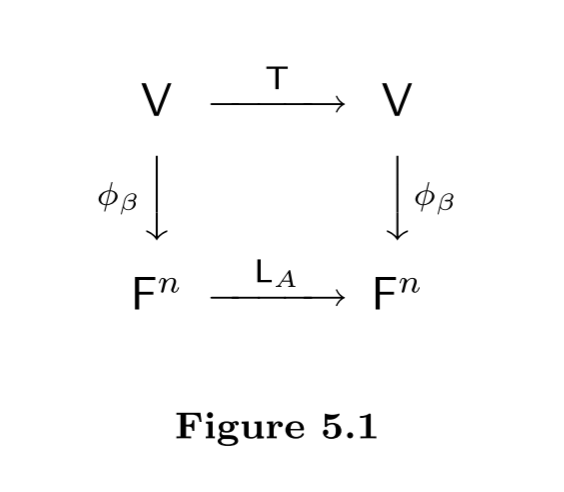
\includegraphics[width=8cm]{images/figure-5-1.png}

Recall that for \(v \in V\), (by \DEF{2.15}) \(\phi_{\beta}(v) = [v]_{\beta}\), the \emph{coordinate vector} of \(v\) \emph{relative to} \(\beta\).

We will show that \(v \in V\) is an eigenvector of \(\T\) corresponding to \(\lambda\) if and only if \(\phi_{\beta}(v)\) is an eigenvector of \(A\) corresponding to \(\lambda\).

Suppose that \(v\) is an eigenvector of \(\T\) corresponding to \(\lambda\).
Then \(v \ne \OV\) and \(\T(v) = \lambda v\) \MAROON{(1)}.
Hence
\begin{align*}
    A \phi_{\beta}(v) & = \LMTRAN_A \phi_{\beta} (v) & \text{by def of left multiplication} \\
        & = \phi_{\beta} \T(v) & \text{by Figure 5.1, the functions ``commute''} \\
        & = \phi_{\beta}(\T(v)) & \text{by def of function composition} \\
        & = \phi_{\beta}(\lambda v) & \text{by \MAROON{(1)}} \\
        & = \lambda \phi_{\beta}(v). & \text{\(\phi_{\beta}\) is linear, in particular}
\end{align*}
And since \(\phi_{\beta}\) is an isomorphism, \(\phi_{\beta}(v) \ne 0 \in F^n\);
hence \(\phi_{\beta}(v)\) is an eigenvector of \(A\) corresponding to \(\lambda\).

Now if \(\phi_{\beta}(v)\) is an eigenvector of \(A\) corresponding to \(\lambda\), then since the argument above is trivially ``reversible'', \(v\) is an eigenvector of \(\T\)
corresponding to \(\lambda\).
(See \EXEC{5.1.14}.)

An equivalent formulation of the result discussed in the preceding paragraph is that for an eigenvalue \(\lambda\) of \(A\) (and hence of \(\T\)),
a vector \(y \in F^n\) is an eigenvector of \(A\) corresponding to \(\lambda\) if and only if \(\phi_{\beta}^{-1}(y)\) is an eigenvector of \(\T\) corresponding to \(\lambda\).

Thus we have \emph{reduced} the problem of finding the eigenvectors \emph{of a linear operator} on a finite-dimensional vector space to the problem of finding the
eigenvectors \emph{of a matrix}.
The next example illustrates this procedure.
\end{remark}

\begin{note}
這邊只是在說,要找一個線性變換的\ eigenvector,可以找這個線性變換「的矩陣代表」的\ eigenvector,該\ vector 其實就是線性變換的某個\ eigenvector 的「座標向量」;
找到該座標向量後把它「轉回」(i.e. 用\ \(\phi_{\beta}^{-1}\) 轉)線性變換的向量即可。
\end{note}

\begin{example} \label{example 5.1.7}
Let \(\T(f(x)) = f(x) + (x + 1)f'(x)\) be the linear operator on \(\POLYRR\) defined in \EXAMPLE{5.1.5},
and let \(\beta\) be the standard ordered basis for \(\POLYRR\).
Recall that \(\T\) has eigenvalues \(1, 2\), and \(3\) and that
\[
    A = [\T]_{\beta} = \begin{pmatrix} 1 & 1 & 0 \\ 0 & 2 & 2 \\ 0 & 0 & 3 \end{pmatrix}.
\]
We consider each eigenvalue separately.

Let \(\lambda_{1}=1\), and define
\
\[
    B_{1}=A-\lambda_{1} I=\left(\begin{array}{lll}
        0 & 1 & 0 \\
        0 & 1 & 2 \\
        0 & 0 & 2
    \end{array}\right).
\]
Then
\[
    x=\left(\begin{array}{l} x_{1} \\ x_{2} \\ x_{3} \end{array}\right) \in \SET{R}^{3}
\]
is an eigenvector corresponding to \(\lambda_{1}=1\) if and only if \(x \ne 0\) and \(x \in \NULL \left( \LMTRAN_{B_{1}} \right)\);
that is, \(x\) is a nonzero solution to the system
\[
    \sysdelim..\systeme{
        x_{2}=0,
        x_{2}+2 x_{3}=0,
        2 x_{3}=0
    }.
\]
Notice that this system has three unknowns, \(x_1, x_2\), and \(x_3\), but one of these, \(x_1\), does not actually appear in the system.
Since the values of \(x_1\) do not affect the system, we assign \(x_1\) a parametric value, say \(x_1 = a\), and solve the system for \(x_2\) and \(x_3\).
Clearly, \(x_2 = x_3 = 0\), and so the eigenvectors \MAROON{of \(A\)} corresponding to \(\lambda_1 = 1\) are of the form
\[
    a \begin{pmatrix} 1 \\ 0 \\ 0 \end{pmatrix} = a e_1
\]
for \(a \ne 0\).
Consequently, the eigenvectors \MAROON{of \(\T\)} corresponding to \(\lambda_1 = 1\) are of the form
\[
    \phi_{\beta}^{-1}\left(a e_{1}\right)=a \phi_{\beta}^{-1}\left(e_{1}\right)=a \cdot 1=a \in \mathcal{P}_2(\SET{R}^2)
\]
for any \(a \ne 0\).
Hence the nonzero constant polynomials are the eigenvectors of \(\T\) corresponding to \(\lambda_1 = 1\).

Next let \(\lambda_2 = 2\), and define
\[
    B_{2}=A-\lambda_{2} I=\left(\begin{array}{lll}
        -1 & 1 & 0 \\
        0 & 0 & 2 \\
        0 & 0 & 1
    \end{array}\right).
\]
It is easily verified that
\[
    \NULL(\LMTRAN_{B_2}) = \left\{ a \begin{pmatrix} 1 \\ 1 \\ 0 \end{pmatrix} : a \in \SET{R} \right\}.
\]
and hence the eigenvectors of \(\T\) corresponding to \(\lambda_2 = 2\) are of the form
\[
    \phi_{\beta}^{-1} \left( a \begin{pmatrix} 1 \\ 1 \\ 0 \end{pmatrix} \right) = a \phi_{\beta}^{-1} (e_1 + e_2) = a (1 + x) = a + x
\]
for \(a \ne 0\).

Finally, consider \(\lambda_{3} = 3\) and
\[
    B_{3}=A-\lambda_{3} I=\left(\begin{array}{rrr}
        -2 & 1 & 0 \\
        0 & -1 & 2 \\
        0 & 0 & 0
    \end{array}\right)
\]
Since
\[
    \NULL\left(\LMTRAN_{B_{3}}\right) = \left\{ a\left(\begin{array}{l} 1 \\ 2 \\ 1 \end{array}\right): a \in \SET{R} \right\},
\]
the eigenvectors of \(\T\) corresponding to \(\lambda_{3}=3\) are of the form
\[
    \phi_{\beta}^{-1}\left(a\left(\begin{array}{l} 1 \\ 2 \\ 1 \end{array}\right)\right)
    = a \phi_{\beta}^{-1}\left(e_{1}+2 e_{2}+e_{3}\right)
    = a \left(1+2 x+x^{2}\right) = a + 2ax + ax^2
\]
for \(a \ne 0\).

For each eigenvalue, select the corresponding eigenvector with \(a = 1 \ne 0\) in the preceding descriptions to obtain \(\gamma = \{ 1, 1 + x, 1 + 2x + x^2 \}\), which is an ordered
basis for \(\POLYRR\) consisting of eigenvectors of \(\T\).
Thus \(\T\) is diagonalizable, and
\[
    [\T]_{\gamma} = \begin{pmatrix} 1 & 0 & 0 \\ 0 & 2 & 0 \\ 0 & 0 & 3 \end{pmatrix}.
\]
\end{example}

We close this section with a \textbf{geometric description} of how a linear operator \(\T\) acts on an eigenvector in the context of a vector space \(V\) over \(\SET{R}\).
(Also see this \href{https://www.youtube.com/watch?v=PFDu9oVAE-g&ab_channel=3Blue1Brown}{video}.)
Let \(v\) be an eigenvector of \(\T\) and \(\lambda\) be the corresponding eigenvalue.
We can think of \(W = \spann(\{ v \})\), the one-dimensional subspace of \(V\) spanned by \(v\), as a line in \(V\) that passes through \(\OV\) and \(v\).
For any \(w \in W, w = cv\) for some scalar \(c\),
and hence
\[
    \T(w) = \T(cv) = c\T(v) = c (\lambda v) = \lambda (c v) = \lambda w;
\]
so \(\T\) acts on the vectors in \(W\) by \textbf{multiplying} each such vector by \(\lambda\).

There are several possible ways for \(\T\) to act on the vectors in \(W\), depending on the value of \(\lambda\).
We consider several cases. (See Figure 5.2.)

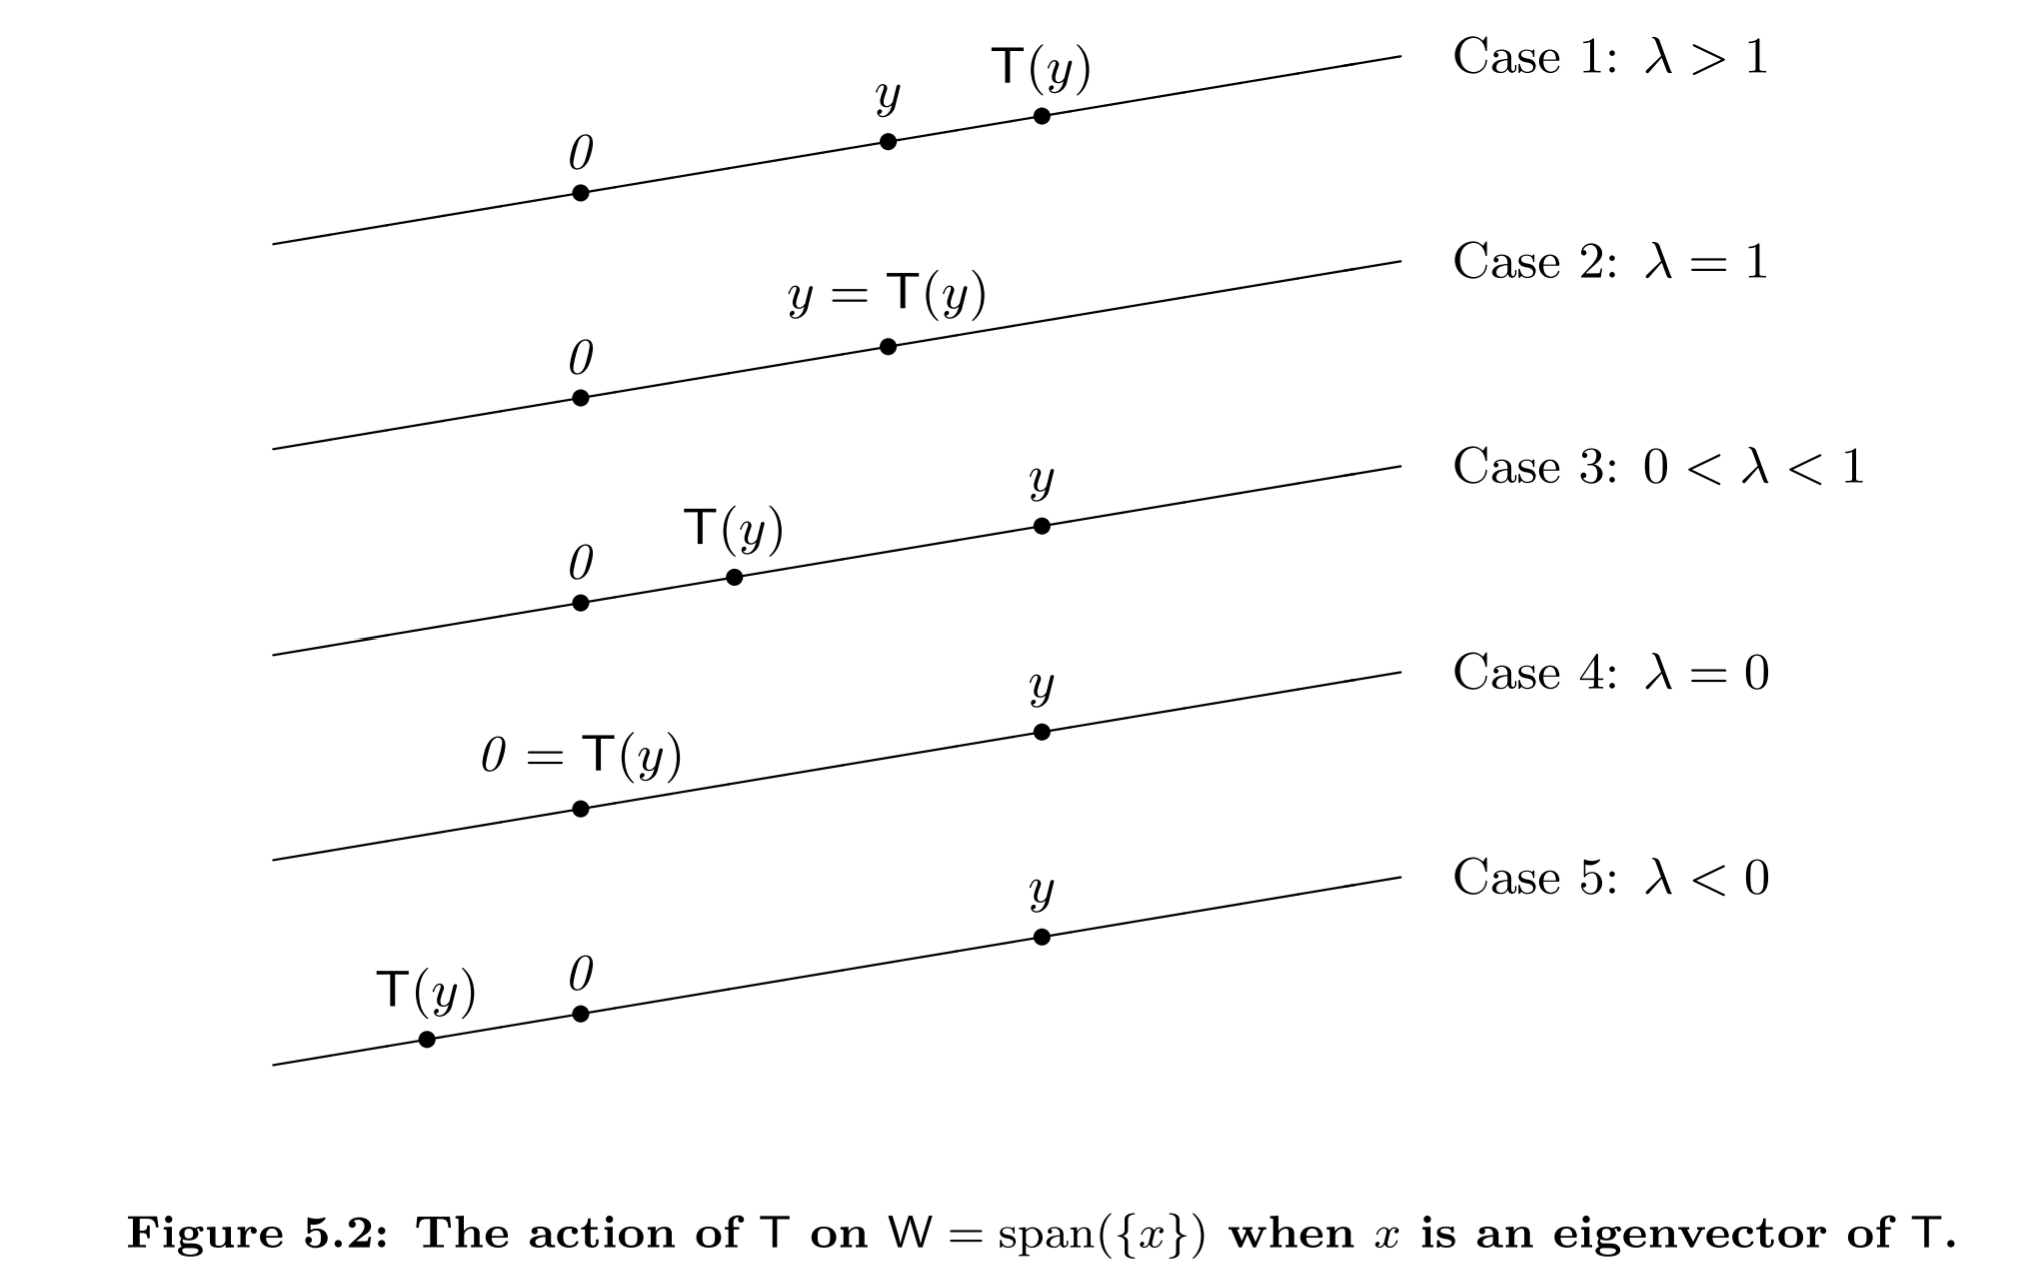
\includegraphics[width=17cm]{images/figure-5-2.png}

\begin{enumerate}
\item[CASE 1.] If \(\lambda > 1\), then \(\T\) moves vectors in \(W\) \emph{farther} from \(\OV\) by a factor of \(\lambda\).
\item[CASE 2.] If \(\lambda = 1\), then \(\T\) acts as the \emph{identity operator} on \(W\).
\item[CASE 3.] If \(\OF < \lambda < 1\), then \(\T\) moves vectors in \(W\) \emph{closer} to \(\OV\) by a factor of \(\lambda\).
\item[CASE 4.] If \(\lambda = \OF\), then \(\T\) acts as the \emph{zero transformation} on \(W\).
\item[CASE 5.] If \(\lambda < \OF\), then \(\T\) \emph{reverses the orientation} of \(W\); that is, \(\T\) moves vectors in \(W\) from one side of \(\OV\) to the other.
\end{enumerate}

To illustrate these ideas, we consider the linear operators in \EXAMPLE{2.1.3}, \EXAMPLE{2.1.4}, and \EXAMPLE{2.1.2}.

For the operator \(\T\) on \(\SET{R}^2\) defined by \(\T(a_1, a_2) = (a_1, -a_2)\), the \emph{reflection} about the \(x\)-axis, \(e_1\) and \(e_2\) are eigenvectors of \(\T\) with corresponding eigenvalues \(1\) and \(-1\), respectively.
Since \(e_1\) and \(e_2\) span the \(x\)-axis and the \(y\)-axis, respectively, \(\T\) \emph{acts as the identity} on the \(x\)-axis and \emph{reverses the orientation}
of the \(y\)-axis.

For the operator \(\T\) on \(\SET{R}^2\) defined by \(\T(a_1, a_2) = (a_1, 0)\), the \emph{projection} on the \(x\)-axis, \(e_1\) and \(e_2\) are eigenvectors of \(\T\) with corresponding eigenvalues \(1\) and \(0\), respectively.
Thus, \(\T\) acts as the identity on the \(x\)-axis and as the \emph{zero operator} on the \(y\)-axis.

Finally, we generalize \EXAMPLE{2.1.2} of this section by considering the operator that \emph{rotates} the plane through the angle, which is defined by
\[
    \T_{\theta}(a_1, a_2) = (a_1 \cos \theta - a_2 \sin \theta, a_1 \sin \theta + a_2 \cos \theta).
\]
Suppose that \(0 < \theta < \pi\).
Then for any nonzero vector \(v\), the vectors \(v\) and \(\T_{\theta}(v)\) are \textbf{not collinear}, and hence \(\T_{\theta}\) maps no one-dimensional subspace of \(\SET{R}^2\) into itself.
But this implies that \(\T_{\theta}\) \emph{has no eigenvectors} and therefore no eigenvalues.
To confirm this conclusion, let \(\beta\) be the standard ordered basis for \(\SET{R}^2\), and note that the \CPOLY{} of \(\T_{\theta}\) is
\[
    \det\left(\left[\T_{\theta}\right]_{\beta}-t I_{2}\right)
    = \det \begin{pmatrix}
        \cos \theta-t & -\sin \theta \\
        \sin \theta & \cos \theta-t
    \end{pmatrix}
    = t^{2} - (2 \cos \theta) t + 1
\]
which has no \textbf{real} zeros because, for \(0 < \theta < \pi\), the discriminant \(4 \cos^2 \theta - 4\) is negative.

\begin{remark} \label{remark 5.1.10}
However, the rotation operator in the previous discussion \emph{does have} eigenvalues when the field is \emph{complex number}, and \(\pm \iu\) are the eigenvalue of this transformation.
In addition, the ``geometric explanation'' in the discussion no longer applies, since it does not correctly describe the ``geometry'' of complex number.
\end{remark}
